\documentclass[t]{sdqbeamer}
%\documentclass[c]{sdqbeamer}

\usepackage{listings}
\usepackage{graphicx}
\usepackage{tabularx}
\usepackage{tikzsymbols}
\usepackage{tikz}
\usepackage{transparent}
\usetikzlibrary{positioning,fit,shapes}
\usepackage[lined,linesnumbered,ruled,noend]{algorithm2e}
\renewcommand{\thealgocf}{}

\hypersetup{
	colorlinks=true,
	urlcolor=kit-orange
}

% set sdqbeamer options
\titleimage{blender-render}
\groupname{} % rendered at the bottom center of each slide
\grouplogo{ae+satres}
\selectlanguage{english}

% define title etc.pp.
\title{Practical SAT Solving}
\subtitle{Lecture 6 \unimp{\normalfont -- Elementary SAT Solving Heuristics, Conflict-Driven Clause Learning}}
\author{\underline{Ashlin Iser}, Dominik Schreiber}
\date{June 1, 2026}

% define commands
\input{l00-commands.tex}

\setlength{\itemsep}{1em}

\begin{document}

\begin{frame}[title white horizontal, picture=logos/blender-render, kitlogo=rgb]
	\titlepage
\end{frame}

\begin{frame}{Overview}
	\begin{block}{Recap.}
		\begin{itemize}\setlength{\itemsep}{1ex}
			\item Lectures 4 \& 5: Applications of SAT Solving
			\item Lecture 3: Elementary SAT Solving Algorithms
			\begin{itemize}
				\item Local Search
				\item Resolution, Saturation, and DP Algorithm
				\item DPLL Algorithm
			\end{itemize}
		\end{itemize}
	\end{block}
	\pause
	\begin{block}{Today's Topics: More on Algorithmic Methods}
		\begin{itemize}\setlength{\itemsep}{1ex}
			\item DPLL: Elementary SAT Solving Heuristics
			\begin{itemize}
				\item Branching Order
				\item Branching Polarity
				\item Restart Strategies
			\end{itemize}
			\item Conflict-Driven Clause Learning (CDCL)
			\begin{itemize}
				\item Implication Graphs
				\item Conflict Analysis
				\item Non-Chronological Backtracking
			\end{itemize}
		\end{itemize}
	\end{block}
\end{frame}

\begin{frame}{DPLL Algorithm: Iterative Variant}
\begin{columns}[T]
\begin{column}{.3\linewidth}
~\\[1em]
\textbf{Decision Heuristics:}~\\[1em]
\begin{itemize}\setlength{\itemsep}{1em}
	\item Branching Order:\\[1ex] Which variable to choose?
	\item Branching Polarity:\\[1ex] Which value to assign?
\end{itemize}
\end{column}
\begin{column}{.6\linewidth}
\begin{algorithm}[H]
\DontPrintSemicolon
\caption{iterativeDPLL(CNF Formula $F$)}
\KwData{Trail (Stack of Literals)}
\BlankLine

\While{not all variables assigned by Trail} {
	\If{unitPropagation(F, Trail) has CONFLICT} {
		$L \leftarrow$ last literal not tried both True and False\;
		\lIf {no such $L$} {\Return UNSAT}
		pop all literals after and including $L$ from Trail\;
		push $\{ L = 0 \}$ on Trail\;
	}
	\Else{ 
		\highlo{$L \leftarrow$ pick an unassigned literal}\;
		push $\{ L = 1 \}$ on Trail \;
	}
}
\Return SAT\;
\end{algorithm}
\end{column}
\end{columns}
\end{frame}

\begin{frame}{Properties of Decision Heuristics}
\textbf{Desired properties}\\[1ex]
\begin{itemize}\setlength{\itemsep}{1ex}
	\item Fast to compute
	\item Gives \highlow{easy sub-problems}\\[3pt]
	\pause
	\begin{itemize}\setlength{\itemsep}{1ex}
		\item Satisfy many clauses
		\item Maximize unit propagation
	\end{itemize}
\end{itemize}
~\\
\pause
\textbf{Types of heuristics}\\[1ex]
\begin{itemize}\setlength{\itemsep}{1ex}
	\item Static vs. Dynamic\\[3pt]
	\begin{itemize}\setlength{\itemsep}{1ex}
		\item Static: Based on formula statistics
		\item Dynamic: Based on formula and current state
	\end{itemize}
	\item Separate vs. Joint\\[3pt]
	\begin{itemize}\setlength{\itemsep}{1ex}
		\item Separate: Choose variable and value independently
		\item Joint: Choose variable and value together
	\end{itemize}
\end{itemize}
\end{frame}

\begin{frame}{Decision Heuristics: Böhm's Heuristic}
\begin{itemize}\setlength{\itemsep}{1ex}
	\item $h_i(x)$: number of clauses of size $i$ containing literal $x$ which are \highl{not yet satisfied}
	\item $H_i(x) := \alpha \operatorname{max}(h_i(x), h_i(\overline{x})) + \beta \operatorname{min}(h_i(x), h_i(\overline{x}))$ \quad (let $\alpha:=1$ and $\beta:=2$, for example)
	\item Select literal $x$ with the \highl{maximal vector $(H_1(x),H_2(x),\dots)$} under lexicographic order
\end{itemize}~\\
\begin{blueblock}{Properties of Böhm's Heuristic}
Goal: \highl{satisfy or reduce size} of many and preferably short clauses\\[1ex]
\begin{itemize}\setlength{\itemsep}{1em}
	\item Separate polarity heuristic (note that $H_i(x) = H_i(\overline x)$)\\[1ex]
		$\rightarrow$ select $x$ if $\sum_i h_i(x) \geq \sum_i h_i(\overline x)$
	\item depends on literal occurrence counts over the not yet satisfied clauses
	\item \href{https://stamm-wilbrandt.de/en/Report_on_a_SAT_competition.pdf}{SAT Competition 1992:} best heuristic for random instances
\end{itemize}
\end{blueblock}
\end{frame}
	
\begin{frame}{Decision Heuristics: Mom's Heuristic}{\textbf{M}aximum \textbf{O}ccurrences in clauses of \textbf{M}inimum \textbf{S}ize}
\begin{itemize}\setlength{\itemsep}{1ex}
	\item $f^*(x)$: how often $x$ occurs in the \highl{smallest not yet satisfied} clauses
	\item Select variable $x$ with a maximum $S(x) = \bigl(f^*(x)+f^*(\overline{x})\bigr) \cdot 2^k + f^*(x) \cdot f^*(\overline{x})$ \quad (let $k:=10$, for example)
\end{itemize}~\\
\begin{blueblock}{Properties of Mom's Heuristic}
Goal: assign variables with \highl{high occurrence in short clauses}\\[1ex]
\begin{itemize}\setlength{\itemsep}{1em}
	\item Separate polarity heuristic\\[1ex]
		$\rightarrow$ for example, select $x$ if $f^*(\overline x) \geq f^*(x)$
	\item depends on literal occurrence counts over the not yet satisfied clauses
	\item Popular in the mid 90s (Find some variants in \href{https://satlecture.github.io/kit2024/references/1995_Freeman_Thesis.ps}{Freeman 1995, pages 39f.})
\end{itemize}
\end{blueblock}
\end{frame}
	
\begin{frame}{Decision Heuristics: Jeroslow-Wang Heuristic}
\begin{itemize}\setlength{\itemsep}{1ex}
	\item Choose the literal $x$ with a maximum $J(x) = \sum_{x \in c,\ c \in F} 2^{-|c|}$
\end{itemize}~\\
\begin{blueblock}{Properties of Jeroslow-Wang Heuristic}
	Goal: assign variables with \highl{high occurrence in short clauses}\\[1ex]
	\begin{itemize}\setlength{\itemsep}{1em}
		\item Considers \highl{all clauses}, but shorter clauses are more important
		\item Separate polarity heuristic\\
		$\rightarrow$ for example, use conflict-seeking polarity heuristic
		\item \highl{Two-sided variant}: choose variable $x$ with maximum $J(x)+J(\overline{x})$\\
		$\rightarrow$ one-sided version works better
	\item Much better experimental results than B{\"o}hm and MOMS
\end{itemize}
\end{blueblock}
\end{frame}
	
\begin{frame}{(R)DLCS and (R)DLIS Heuristics}{(\textbf{R}andomized) \textbf{D}ynamic \textbf{L}argest (\textbf{C}ombined | \textbf{I}ndividual) \textbf{S}um}
\begin{itemize}\setlength{\itemsep}{1ex}
	\item based on positive $C_P(x)$ and negative occurences $C_N(x)$ of variable $x$
	\item used in the famous SAT solver \highl{GRASP} in 2000
\end{itemize}~\\
\begin{blueblock}{Properties of (R)DLCS and (R)DLIS Heuristics}
\begin{itemize}\setlength{\itemsep}{1em}
	\item \highl{Dynamic}: Take the \highl{current partial assignment} into account
	\item \highl{Combined}: select $x$ with maximal $C_P(x)+C_N(x)$
	\item \highl{Individual}: select $x$ with maximal $\operatorname{max}(C_P(x),C_N(x))$
	\item \highl{Randomized}: randomly select variable among the best
\end{itemize}
\end{blueblock}
\end{frame}
	
\iffalse
\begin{frame}{LEFV Heuristic}
\textbf{L}ast \textbf{E}ncountered \textbf{F}ree \textbf{V}ariable:
\begin{itemize}
	\item During unit propagation save the \highl{last unassigned variable} you see
	\item If the variable is \highl{still unassigned} at decision time, use it; \\
	otherwise, choose a \highl{random variable}
	\item \highl{Very fast computation}: constant memory and time overhead
	\begin{itemize}
	\item Requires 1 int variable (to store the last seen unassigned variable)
	\end{itemize}
	\item Maintains \highl{search locality}
	\item Works well for \highlo{Pigeon Hole} and similar formulas
\end{itemize}
\end{frame}
\fi

\begin{frame}{Recap}
\begin{block}{Decision Heuristics}
\begin{itemize}\setlength{\itemsep}{1ex}
	\item Böhm's Heuristic
	\item Mom's Heuristic
	\item Jeroslow-Wang Heuristic
	\item (R)DLCS and (R)DLIS Heuristics
\end{itemize}
\end{block}
\begin{block}{Next up}
	Restart Strategies
\end{block}
\end{frame}
		
\begin{frame}{Restarts Strategies: Motivation}
\vspace{-1em}
Given $n$ runs of \highl{randomized DPLL search}, what is the \highl{average number of backtracks} per run?\\[2em]
\begin{columns}
\begin{column}{0.6\textwidth}
	\centering
		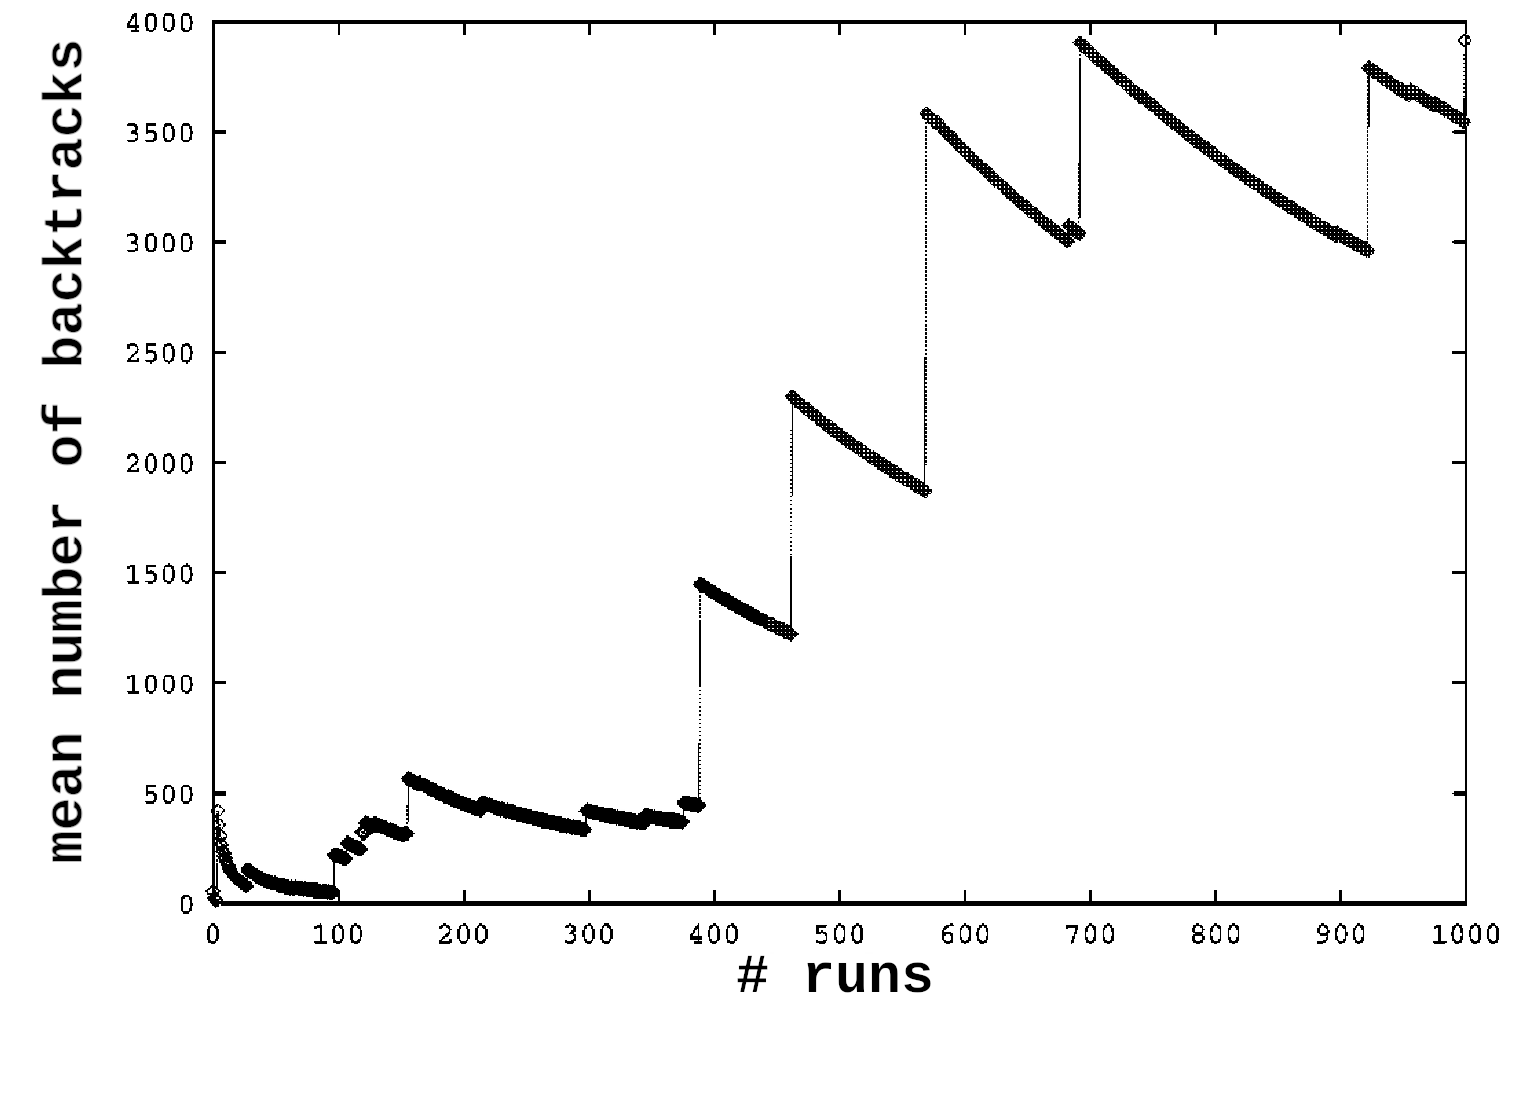
\includegraphics[width=.7\textwidth]{figures/l04/heavy-tail-1}\\
		\highlow{Heavy-tailed distribution}\\
		% $P[X > x] \sim C \cdot x^{-\alpha}, \quad C > 0, \alpha \in (0,2)$
\end{column}
\begin{column}{0.4\textwidth}
	\centering
	{
	\transparent{0.5}
	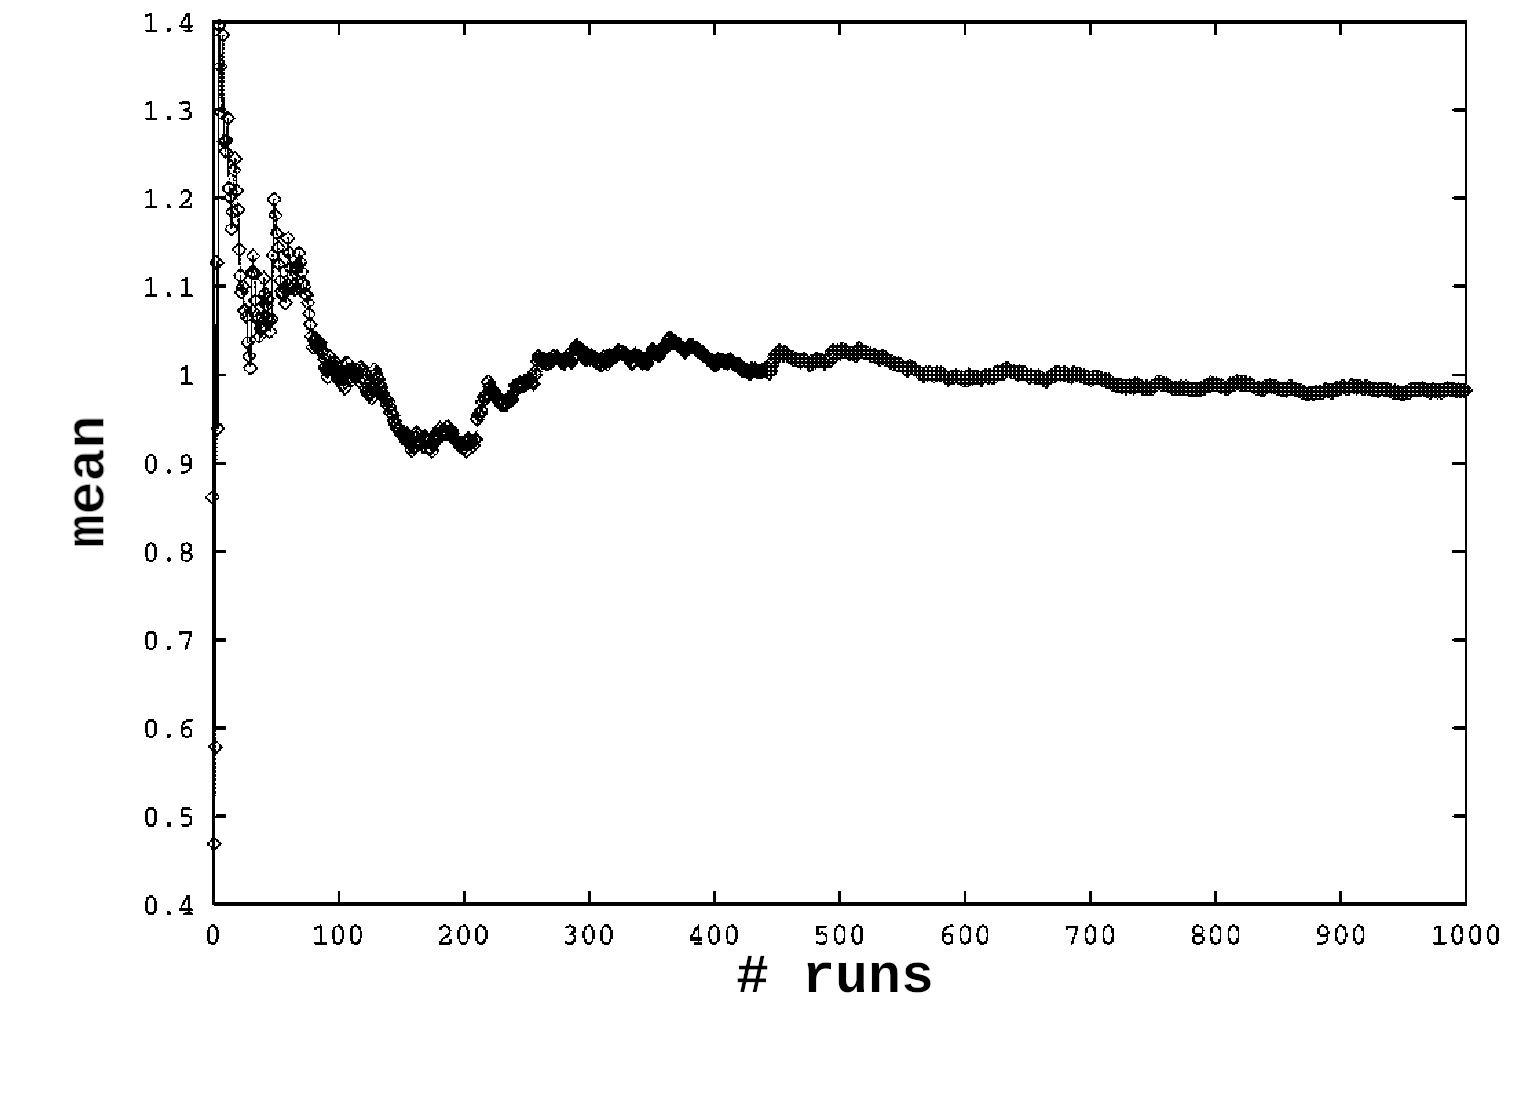
\includegraphics[width=.7\textwidth]{figures/l04/heavy-tail-2}\\
	\textit{For Reference:}\\ Standard distribution\\
	}
	% $P[X > x] \sim \frac{1}{x\sqrt{2\pi}}e^{-x^2/2}$
\end{column}
\end{columns}~\\[2em]
\hfill\small\href{https://doi.org/10.1023/A:1006314320276}{[Gomes et al. 2000]}
\end{frame}

\begin{frame}{Restart Strategies}
\vspace{-1em}
Clear the partial assignment and backtrack to the root of the search tree.\\[1ex]
\begin{itemize}\setlength{\itemsep}{1ex}
	\item Recover from bad branching decisions
	\item Solve more instances on average
	\item Might decrease performance on easy instances
\end{itemize}~\\[1ex]
\begin{blueblock}{When to Restart?}
\begin{itemize}\setlength{\itemsep}{1em}
	\item After some number of conflicts / backtracks
	\item The intervals between restarts should increase to guarantee \highlow{completeness}\\[1ex]
	\begin{itemize}\setlength{\itemsep}{1ex}
		\item Linear increase: too slow
		\item Exponential increase: ok, with small exponent
		\item MiniSat: $k$-th restart happens after $100 \times 1.1^k$ conflicts
	\end{itemize}
\end{itemize}
\end{blueblock}
\end{frame}

\begin{frame}{Restart Strategies: Inner / Outer Pattern (MiniSat)}
\begin{columns}[T]
\begin{column}{0.5\textwidth}
	\centering
	\visible<2>{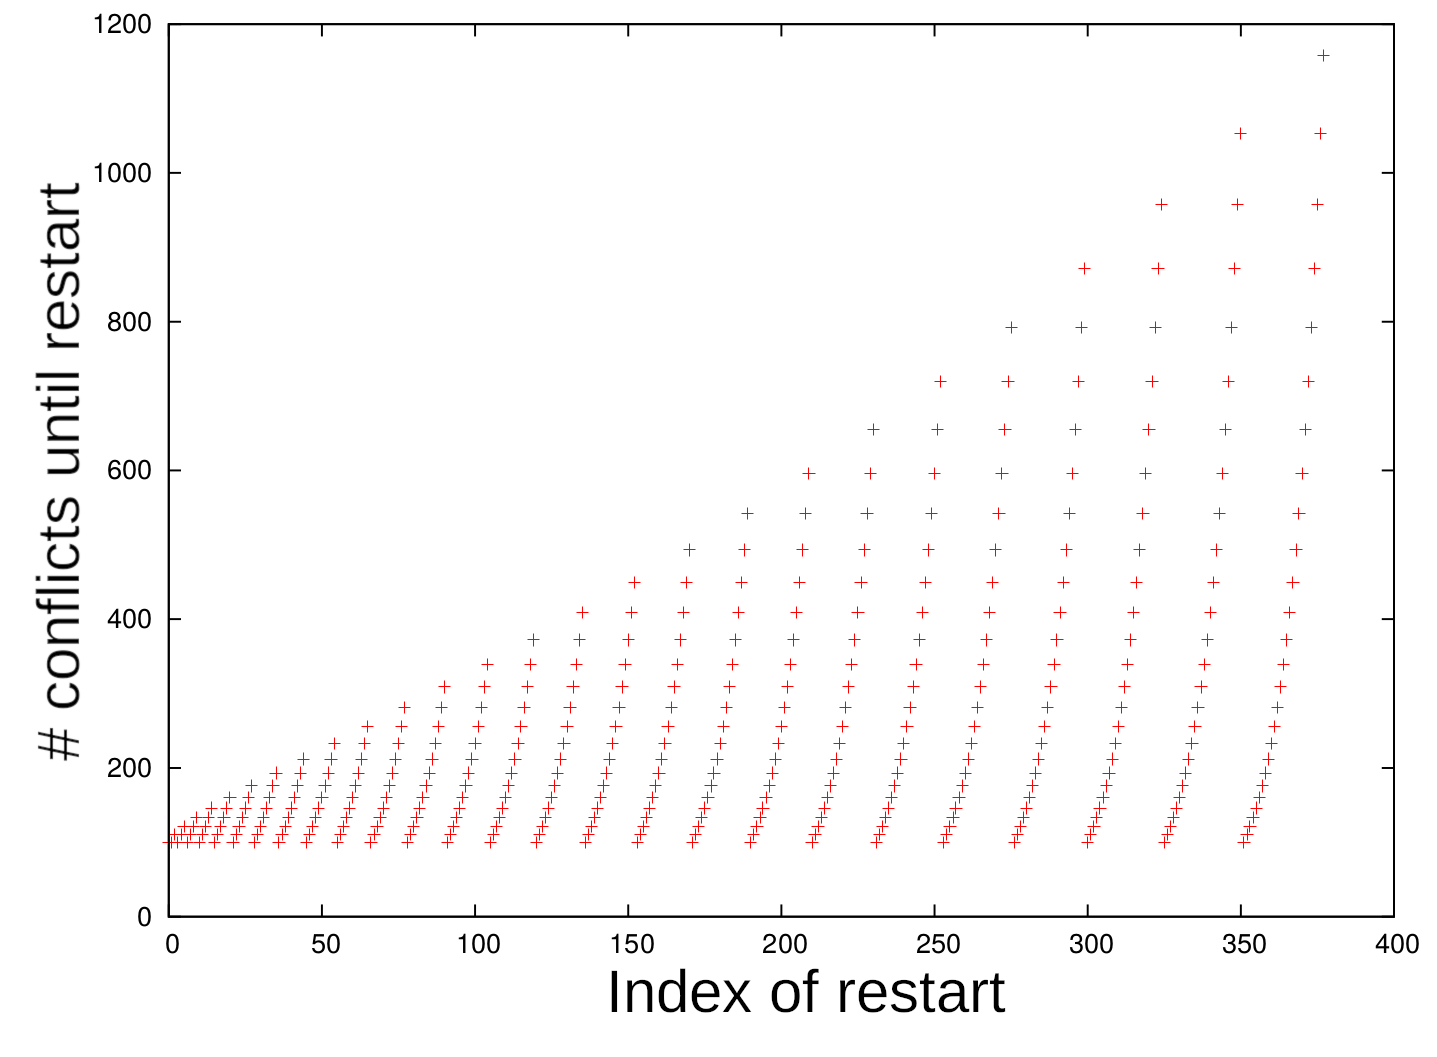
\includegraphics[width=\textwidth]{figures/l04/restart-inout-legend}}
\end{column}
\begin{column}{0.45\textwidth}
\begin{algorithm}[H]
	\DontPrintSemicolon
	\caption{Inner / Outer}
	\KwData{int inner = 100, outer = 100}
	\BlankLine
	\While{true} {
		run DPLL() with conflict-limit $inner$\;
		restarts++\;
		\If{inner $\geq$ outer} {
			outer *= 1.1\;
			inner = 100\;
		}
		\Else{
			inner *= 1.1\;
		}
	}
\end{algorithm}
\end{column}
\end{columns}
\end{frame}

\begin{frame}{Restart Strategies: Luby Sequence}
\begin{blueblock}{Theorem \href{https://doi.org/10.1016/0020-0190(93)90029-9}{[Luby et al, 1993]}}
	Consider a \highlow{Las Vegas} algorithm $A$ (i.e., correct but with \highlow{random run time}) and a restart strategy $S = \langle t_1, t_2, \ldots \rangle$ (i.e., run $A$ for time $t_1$, then for time $t_2$, etc.).	
	Up to a constant factor, the Luby sequence is the \highlow{best possible universal strategy to minimize the expected run time} until a run is successful.
	\begin{align*}
		Luby = u \cdot (t_i)_{i \in \mathbb{N}} \quad \text{with} \quad t_i = \begin{cases}
			2^{k-1} & \text{if $i = 2^k - 1$} \\
			t_{i-2^{k-1}+1} & \text{if $2^{k-1} \leq i \leq 2^k -1$} \\
		\end{cases}
	\end{align*}~\\[1em]
	\textbf{Example: }$1, 1, 2, 1, 1, 2, 4, 1, 1, 2, 1, 1, 2, 4, 8, \dots$
\end{blueblock}
\end{frame}
		
\begin{frame}{Restart Strategies: Luby Sequence}
\begin{columns}[T]
\begin{column}{0.5\textwidth}
	\centering
	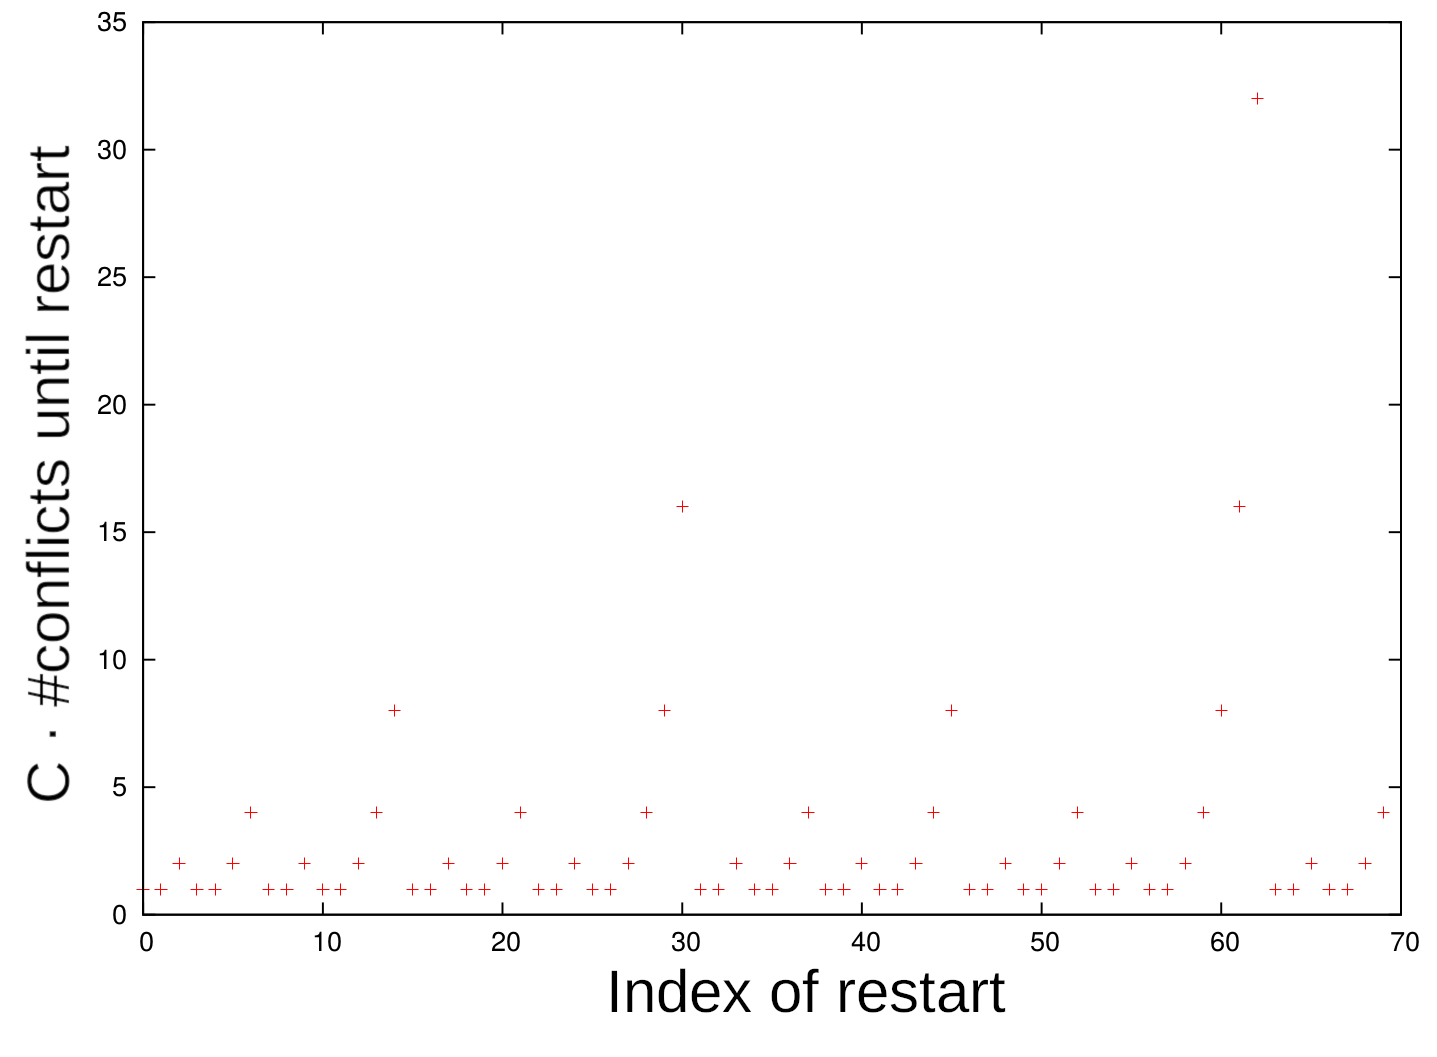
\includegraphics[width=\textwidth]{figures/l04/restart-luby-legend}
\end{column}
\begin{column}{0.45\textwidth}
\begin{algorithm}[H]
	\DontPrintSemicolon
	\caption{Luby Sequence}
	\KwIn{int $i \geq 1$ \tcp*[f]{index of the $i$-th restart}}
	\BlankLine
	\tcc{determine smallest $k$ with $i \leq 2^k - 1$, i.e. $k = \lceil \log_2(i+1) \rceil$}
	$k \gets 1$\;
	\While {$i > (1 \ll k) - 1$} {
		$k \gets k + 1$
	}
	\BlankLine
	\tcp{emit peak}
	\If {$i == (1 \ll k) - 1$} {
		\Return $1 \ll (k-1)$
	}
	\BlankLine
	\tcp{recurse into first half}
	\Return Luby($i - (1 \ll (k-1)) + 1$)
\end{algorithm}
\end{column}
\end{columns}~\\[1ex]
Example usage in SAT solvers: Run DPLL() with conflict-limit $512 \cdot$ \text{Luby}(++restarts)
\end{frame}
		
\begin{frame}{Restart Strategies: Luby Sequence}
\begin{blueblock}{Luby Sequence: Reluctant Doubling}
A more efficient implementation of the Luby sequence invented by Donald Knuth.\\[1ex]
Use the $v_n$ of the following pairs $(u_n, v_n)$:
\begin{align*}
(u_1, v_1) &\;:=\; (1,\, 1) \\[0.4ex]
(u_{n+1}, v_{n+1}) &\;:=\;
\bigl(u_n \mathbin{\&} (-u_n)\bigr) = v_n
\;\;\mathrel{?}\;\; (u_n{+}1,\, 1)
\;\;\mathrel{:}\;\; (u_n,\, 2 \cdot v_n)
\end{align*}~\\[1ex]
\textbf{Example: }$(1,\mathbf{1}), (2,\mathbf{1}), (2,\mathbf{2}), (3,\mathbf{1}), (4,\mathbf{1}), (4,\mathbf{2}), (4,\mathbf{4}), (5,\mathbf{1}), \ldots$\\[1em]
\textbf{Intuition: }$u_n$ counts which ``run'' we are in; $v_n$ doubles inside that run until it reaches the lowest set bit of $u_n$, at which point Luby's recursive structure demands a reset.
The $u \mathbin{\&} (-u)$ part is a one-instruction way to isolate that bit.
\end{blueblock}
\end{frame}


\begin{frame}{Branching Polarity: Phase Saving}
\textbf{Observation:} Frequent restarts can \highlow{destroy useful work} on satisfiable instances --- after a restart, the solver may pick the opposite polarity and re-explore parts of the search space it had already shown to be consistent.\\[1em]
\begin{blueblock}{Phase Saving / Assignment Caching \hfill \href{http://reasoning.cs.ucla.edu/rsat/}{[RSAT, 2006]}}
	\vspace{0.3em}
	\begin{columns}[T]
		\begin{column}{0.02\textwidth}\end{column}
		\begin{column}{0.62\textwidth}
\textbf{Idea:} Remember the \highlow{last assigned value} of each variable and reuse it the next time the variable is branched on (after a restart or backtrack).\\[1ex]
\begin{itemize}\setlength{\itemsep}{0.8em}
	\item Preserves consistent assignments across restarts
	\item \highlow{Stabilizes} the positive effect of frequent restarts
	\item Especially effective combined with \highlow{non-chronological backtracking} (next topic): the solver can jump back over a satisfied component and later restore it from cache
\end{itemize}
\end{column}
\begin{column}{0.27\textwidth}
\centering
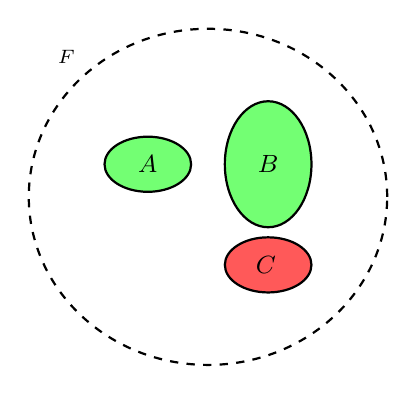
\begin{tikzpicture}[
		cluster/.style = {ellipse, draw, thick, minimum width=1.1cm, minimum height=0.7cm, font=\small},
		formula/.style = {ellipse, draw, thick, dashed, inner sep=4pt, font=\small\itshape}
	]
	\node[cluster, fill=green!55] (A) {$A$};
	\node[cluster, fill=green!55, right=0.4cm of A, minimum height=1.6cm] (B) {$B$};
	\node[cluster, fill=red!65,  below=0.1cm of B] (C) {$C$\,\blitz};
	\node[formula, fit=(A) (B) (C), inner sep=8pt, label={[font=\scriptsize\itshape]above left:$F$}] {};
\end{tikzpicture}\\[0.8ex]
\begin{flushleft}\footnotesize
$A$, $B$, $C$: \highlow{clusters of variables};\\ $F$: the whole formula.\\[0.3ex]
\textcolor{green!55!black}{\textbf{green}} = satisfied component,\\ \textcolor{red!75!black}{\textbf{red}} = current conflict.\\[0.3ex]
Phase cache restores $A$, $B$ \highlow{without re-search}.
\end{flushleft}
\end{column}
		\begin{column}{0.02\textwidth}\end{column}
\end{columns}
\vspace{0.3em}
\end{blueblock}
\end{frame}

\begin{frame}{Recap}
	\begin{block}{Decision Heuristics}
		B\"ohm, MOMS, Jeroslow-Wang, (R)DLCS / (R)DLIS
	\end{block}
	\begin{block}{Restart Strategies}
		\begin{itemize}\setlength{\itemsep}{1ex}
			\item Inner / Outer Pattern
			\item Luby Sequence / Reluctant Doubling
			\item Phase Saving / Assignment Caching
		\end{itemize}
	\end{block}
	\begin{block}{Next up}
		Clause Learning
	\end{block}
\end{frame}


\begin{frame}{DPLL: Chronological Backtracking}
\begin{columns}[T]
\begin{column}{.45\textwidth}
	\begin{flalign*}
	\bigl\{ & \{A, B\}, \{B, C\}, \{\neg A, \neg X, Y \}, &&\\
	& \{\neg A, X, Z\}, \{\neg A, X, \neg Z\}, &&\\
	& \{\neg A, \neg Y, Z\}, \{\neg A, \neg Y, \neg Z \} \bigr\} \tag{Formula} &&\\[1em]
	\only<1>{ & \highlo{A, B, C, X}, Y, Z \tag{Trail} &&\\[1em]} 
	\only<2>{ & \highlo{A, B, C, \neg X}, Z \tag{Trail} &&\\[1em]}
	\only<1>{& \color{myred} \{\neg A, \neg Y, \neg Z \} && \tag{Conflicting Clause}}
	\only<2>{& \color{myred} \{\neg A, X, \neg Z\} && \tag{Conflicting Clause}}
	\end{flalign*}~\\[-2em]
	\only<3>{
	\textbf{Observation:}
	Conflicting clauses $\{\neg A, \neg Y, \neg Z \}$, $\{\neg A, X, \neg Z\}$ constrain only a fraction of the trail ($B$ and $C$ irrelevant)\\[1em]
	How to find out which assignments on the trail are \highlow{relevant for the actual conflict} and immediately backtrack to $A$?
	}
\end{column}
\begin{column}{.45\textwidth} 
	\centering
	\begin{tikzpicture}[node distance=2em]
		\node at (current page.north east) (a) { A };
		\node[below left=2ex of a] (b0) { B };
		\node[right=5em of b0] (b1) { [B=1] };
		\node[below=of b0] (c0) { C };
		\node[below=of c0] (x0) { X };
		\node[below=of x0, xshift=-2em] (y0) { [Y=1] };
		\node[below=2ex of y0] (z1) { [Z=1,Z=0]\blitz };
		\node[below=of x0, xshift=2em] (z0) { [Z=1,Z=0]\blitz };

		\draw[->] (a) -- (b0) node [near start, left] {1} -- (c0) node [near start, left] {1} -- (x0) node [near start, left] {1} -- (y0) node [near start, left] {1} -- (z1);
		\draw[->] (x0) -- (z0) node [near start, right] {0};
		\draw[->] (a) -- (b1) node [near start, right] {0};

		\only<1-2> {
			\node[below=of b1] (c1) { [C=1] };
			\node[below=of c1] (x1) { X };
			\node[right=4em of x1] (x2) { X };
			\node[right=1ex of z0] (l0) {\blitz};
			\node[right=1ex of l0] (l1) {\blitz};
			\node[right=3ex of l1] (l2) {\blitz};
			\node[right=2ex of l2] (l3) {\blitz};
			\draw[->] (c0) -- (x1) node [near start, right] {0} -- (l0) node [near start, left] {1};
			\draw[->] (c0) -- (x1) node [near start, right] {0} -- (l1) node [near start, right] {0};
			\draw[->] (b0) -- (c1) node [near start, right] {0} -- (x2) -- (l2) node [near start, left] {1};
			\draw[->] (b0) -- (c1) node [near start, right] {0} -- (x2) -- (l3) node [near start, right] {0};
		}

		\begin{scope}[every path/.style={->, draw=myblue, ultra thick}]
			\only<1> { \draw (a) -- (b0) -- (c0) -- (x0) -- (y0) -- (z1); }
			\only<2> { \draw (a) -- (b0) -- (c0) -- (x0) -- (z0); }
			\only<3> { \draw (a) -- (b1); }
		\end{scope}
	\end{tikzpicture}
\end{column}
\end{columns}
\end{frame}


\begin{frame}{Implication Graph}
\textbf{Idea:} Make the \highlow{causal structure} of unit propagation explicit, so we can read off \emph{why} a conflict occurred and \emph{which earlier decisions are to blame}.\\[1em]
\begin{blueblock}{Definition: Implication Graph}
Given a formula $F$, assignment trail $T$, and conflicting clause $C$,\\
the implication graph is a DAG $G=(V \cup \{ \text{\blitz} \},E)$ where\\[1ex]
\begin{itemize}\setlength{\itemsep}{0.8em}
	\item each vertex $[\ell_i, d_i]$ corresponds to a literal $\ell_i$ on the trail together with its \highlow{decision level} $d_i$
	\item the special vertex \blitz{} represents the \highlow{conflict};\\[1ex]
	all literals of $C$ have edges to \blitz{}
	\item there is an edge $\bigl([\ell_i, d_i], [u_{i,j}, d_i]\bigr)$ whenever $u_{i,j}$ was propagated by a clause containing $\lnot\ell_i$\\[1ex] (i.e., $\ell_i$ is one of the \highlow{reasons} for $u_{i,j}$)
\end{itemize}
\end{blueblock}
\end{frame}


\begin{frame}{Example: Implication Graph}
Implication graph for the conflicting state under the trail $A, B, C, X, Y, Z$.\\
Node labels show a variable assignment with its \highlow{decision level}; edge labels denote the \highlo{propagating clause}.
\begin{columns}[T]
\begin{column}{0.32\textwidth}
~\\[1ex]
\textbf{Reading the graph:}
\begin{itemize}\setlength{\itemsep}{0.5em}
	\item \highlo{Source} $A$ is the only decision literal causing the conflict ($B$, $C$ are irrelevant).
	\item \highlo{Sink} \blitz{} is the conflict; its in-edges come from the conflicting clause $\{\neg A, \neg Y, \neg Z\}$ (clause~7).
	\item Any \highlo{cut} separating $A$ from \blitz{} yields a \highlo{candidate learned clause}.
\end{itemize}~\\[0.4em]
\end{column}
\begin{column}{0.35\textwidth} 
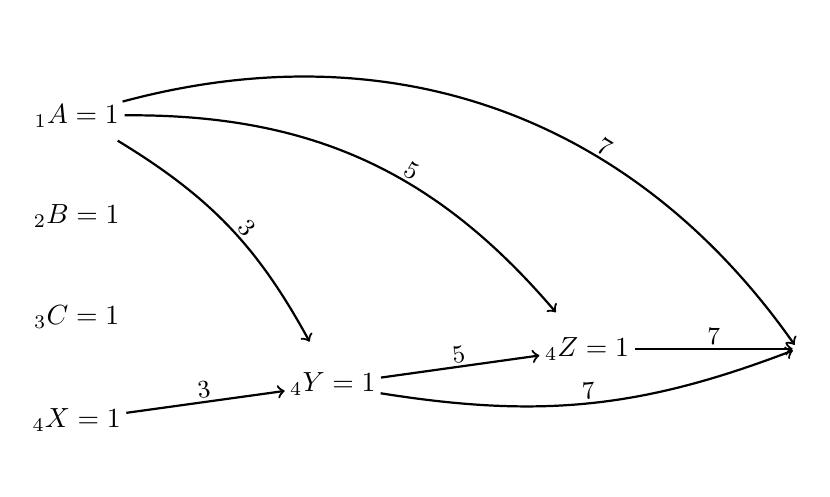
\begin{tikzpicture}[->, thick, node distance=0.05cm and 2cm,
		every edge/.append style={shorten >=1pt, shorten <=1pt},
		every node/.append style={inner sep=1pt},
		elbl/.style={font=\small, inner sep=1pt, sloped, above, anchor=south}]
\node (A) [circle] { $_{\highlow 1}A=1$ };
\node (B) [circle, below=of A] { $_{\highlow 2}B=1$ }; 
\node (C) [circle, below=of B] { $_{\highlow 3}C=1$ };
\node (X) [circle, below=of C] { $_{\highlow 4}X=1$ };
\node (Y) [circle, right=of X, yshift=0.45cm] { $_{\highlow 4}Y=1$ };
\node (Z) [circle, right=of Y, yshift=0.45cm] { $_{\highlow 4}Z=1$ };
\node (empty) [circle, right=of Z] { \blitz };

\draw (X) -- (Y) node [elbl, pos=0.5] {\highlo 3 };
\draw (Y) -- (Z) node [elbl, pos=0.5] {\highlo 5 };
\draw (Z) -- (empty) node [elbl, pos=0.5] {\highlo 7 };
\draw (A) to[bend left=15] node [elbl, pos=0.55] {\highlo 3 } (Y);
\draw (A) to[bend left=25] node [elbl, pos=0.6] {\highlo 5 } (Z);
\draw (A) to[bend left=35] node [elbl, pos=0.65] {\highlo 7 } (empty);
\draw (Y) to[bend right=15] node [elbl, pos=0.5] {\highlo 7 } (empty);
\end{tikzpicture}%
\end{column}%
\begin{column}{.23\textwidth} 
\begin{align*}
\{ & \{A, B\}, \tag{\highlo{1}}\\
& \{B, C\}, \tag{\highlo{2}}\\
& \{\neg A, \neg X, Y \}, \tag{\highlo{3}}\\
& \{\neg A, X, Z\}, \tag{\highlo{4}}\\
& \{\neg A, \neg Y, Z\}, \tag{\highlo{5}}\\
& \{\neg A, X, \neg Z\}, \tag{\highlo{6}}\\
& \{\neg A, \neg Y, \neg Z \} \}\tag{\highlo{7}}
\end{align*}%
\end{column}%
\end{columns}~\\[1ex]
\textbf{Example cut $\{\neg A, \neg X\}$:}
derive by resolution $(7 \circ_Z 5) \circ_Y 3$;\\
Learning it forbids the same partial assignment from being revisited.
\end{frame}

\begin{frame}{Conflict Analysis: Implementation}
Implement the trail as a \highlo{stack of literals}, each paired with a pointer to its \highlo{reason clause} (\emph{null} for decisions) and its \highlo{decision level}. On a conflict, walk the trail top-down and \highlow{resolve} the conflicting clause against the reason clauses of the involved literals until only one literal of the current decision level remains.\\[1em]
\textbf{Example:} Conflict on clause $\{\lnot A, \lnot Y, \lnot Z \}$ at decision level~4.\\[1ex]
\begin{columns}[T]
\begin{column}{.32\linewidth}
	\centering
	\begin{tabular}{@{}c@{\;\;}c@{\;\;}l@{}}
	\textbf{Var.} & \textbf{Lvl.} & \textbf{Reason} \\\hline
	{\color{myred}\blitz} & 4 & {\color{myred}$\{\lnot A, \lnot Y, \lnot Z \}$} \\
	\highlo{Z} & 4 & $\{\lnot A, \lnot Y, Z \}$ \\
	\highlo{Y} & 4 & $\{\lnot A, \lnot X, Y \}$ \\
	X & 4 & \emph{null}\\
	C & 3 & \emph{null}\\
	B & 2 & \emph{null}\\
	A & 1 & \emph{null}\\
	\end{tabular}
\end{column}
\begin{column}{.62\linewidth}
	\textbf{Trail Resolution:}
	\setlength{\leftmargini}{1.2em}
	\begin{itemize}\setlength{\itemsep}{0.6em}
	\item Start from the conflicting clause:\\[2pt]
		$\{\lnot A, \lnot Y, \lnot Z\}$
	\item Resolve on \highlo{$Z$} with reason of $Z$:\\[2pt]
		$\{\lnot A, \lnot Y, \lnot Z\} \mathbin{\otimes_{\highlo Z}} \{\lnot A, \lnot Y, Z\} \;=\; \{\lnot A, \lnot Y\}$
	\item Resolve on \highlo{$Y$} with reason of $Y$:\\[2pt]
		$\{\lnot A, \lnot Y\} \mathbin{\otimes_{\highlo Y}} \{\lnot A, \lnot X, Y\} \;=\; \{\lnot A, \lnot X\}$
	\item Stop: only one literal ($\lnot X$) of level~4 remains.\\[2pt]
		\highlow{Learned clause:} $C = \{\lnot A, \lnot X\}$
	\end{itemize}
\end{column}
\end{columns}
\end{frame}


\begin{frame}{Conflict Analysis: Unit Implication Points (UIP)}
\begin{columns}[T]
\begin{column}{0.45\textwidth}
Several possibilities to learn a clause from an implication graph exist.\\[1em]
	\begin{itemize}\setlength{\itemsep}{1em}
		\item UIP is a dominator in the implication graph (restricted to variables assigned at the current
		decision level)
		\item A node $v$ is a dominator for \blitz, if all paths to \blitz contain $v$
		\item FirstUIP: ``first'' dominator (seen from conflict side)
	\end{itemize}
\end{column}
\begin{column}{0.5\textwidth}
	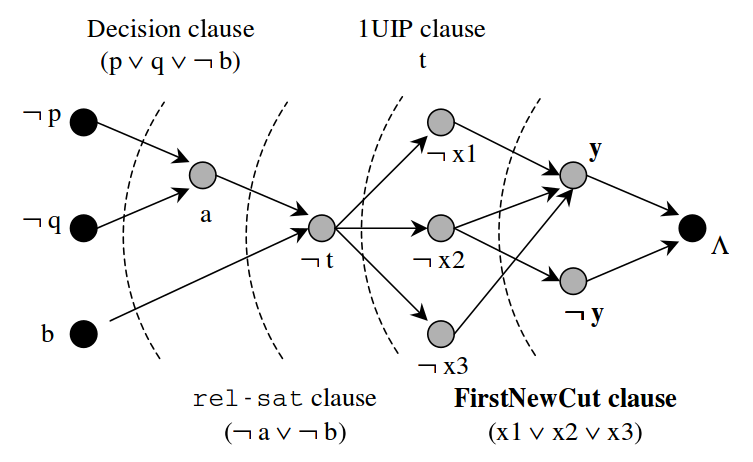
\includegraphics[width=\linewidth]{figures/l04/implicationgraphcuts.png}
\end{column}
\end{columns}~\\[1em]
\hfill\href{http://ijcai.org/Proceedings/03/Papers/171.pdf}{[Beame et al, 2003]}
\end{frame}
			
			
\begin{frame}{Conflict Analysis: 1-UIP Learning}
Resolve the conflicting clause and reason clauses until only a single literal of the current decision level remains.\\[1em]
\textbf{Advantage:}
\begin{itemize}\itemsep1em
	\item Stopping at a UIP always leads to an asserting clause.
	\item A clause is asserting if all literals are false except one, which is unassigned.
	\item Algorithm becomes simpler: backtrack until clause becomes asserting.
	\item The backtrack level is always the second highest level in a conflict clause.
\end{itemize}
\end{frame}


\begin{frame}{Non-chronological Backtracking}
1-UIP learning changes the decision tree in our example like this:~\\[1ex]
\begin{columns}[T]
\begin{column}{0.4\textwidth} 
\begin{tikzpicture}[node distance=2em]
\begin{scope}[node distance=1.5em]
\node at (current page.north east) (a) { A };
\node[below left=of a, xshift=-2em] (b0) { B };
\node[below right=of a, xshift=2em] (b1) { [B=1] };

\node[below=of b0] (c0) { C };
\node[below=of c0] (x0) { X };

\node[below=of x0] (y0) { [Y=1] };
\node[below=of y0] (z1) { [Z=1, Z=0]\blitz };

\node[below=of a] (y1) { [Y=0]};
\node[below=of y1] (x1) { [X=0]};
\node[below=of x1] (z0) { [Z=1, Z=0]\blitz };
\end{scope}

\begin{scope}[every node/.append style = {font=\footnotesize, inner sep=2pt}]
\draw[->] (a) -- (b0) node [near start, left] {1~~};
\draw[->] (b0) -- (c0) node [near start, left] {1};
\draw[->] (c0) -- (x0) node [near start, left] {1};
\draw[->] (x0) -- (y0) node [near start, left] {1};
\draw[->] (y0) -- (z1) node [near start, left] {1};

\draw[->] (a) -- (y1) node [near start, left] {1};
\draw[->] (y1) -- (x1);
\draw[->] (x1) -- (z0);

\draw[->] (a) -- (b1) node [near start, right] {~~0};

\only<1> {
\draw[->, myblue, line width=1.2pt] (a) -- (b0);
\draw[->, myblue, line width=1.2pt] (b0) -- (c0);
\draw[->, myblue, line width=1.2pt] (c0) -- (x0);
\draw[->, myblue, line width=1.2pt] (x0) -- (y0);
\draw[->, myblue, line width=1.2pt] (y0) -- (z1);
}
\only<2> {
\draw[->, myblue, line width=1.2pt] (a) -- (y1);
\draw[->, myblue, line width=1.2pt] (y1) -- (x1);
\draw[->, myblue, line width=1.2pt] (x1) -- (z0);
}
\end{scope}
\end{tikzpicture}
\end{column}%
\begin{column}{0.6\textwidth} 
\begin{align*}
F = \{ & \{A, B\}, \{B, C\}, \\
& \{\neg A, \neg X, Y \}, \\
& \{\neg A, X, Z\}, \\
& \{\neg A, \neg Y, Z\}, \\
& \{\neg A, X, \neg Z\}, \\
& \{\neg A, \neg Y, \neg Z \}%
\only<2>{\\ & {\color{myred} \{\neg A, \neg Y \} }} %
\}
\end{align*}%
Trail: 
\only<1>{$A, B, C, X, Y, Z$}
\only<2>{$A, \neg Y, \neg X, Z$}
\\
Conflicting Clause: 
\only<1>{\color{myred} $\{\neg A, \neg Y, \neg Z \}$}
\only<2>{{\color{myred} $\{\neg A, X, \neg Z\}$}}
{\only<1>{\\ {\color{black} Conflict Clause (1UIP): }{\color{myred} $\{\neg A, \neg Y \}$ }}}
\end{column}
\end{columns}
\end{frame}


\begin{frame}{Clause Learning: Further Reading}
\textbf{Beyond 1-UIP:} apply the UIP idea on \highlow{every} decision level (\highlo{all-UIP}) so that each level contributes at most one literal to the learned clause.
This can produce much shorter clauses. 
But, unlike 1-UIP, it may also \highlow{introduce new literals} on lower levels, so the clause could actually grow.\\[1em]
\begin{itemize}\itemsep1em
	\item \href{https://doi.org/10.1007/978-3-030-51825-7_3}{\highlo{Feng \& Bacchus, SAT 2020} -- Clause Size Reduction with all-UIP Learning}\\[1ex]
	First \highlow{good background overview of learning variants}, then introduces all-UIP shrinking.
	Naively too expensive and prone to enlarging the clause, so they \highlow{guard it} with several heuristics.

	\item \href{https://doi.org/10.1007/978-3-030-80223-3_12}{\highlo{Fleury \& Biere, SAT 2021} -- Efficient All-UIP Learned Clause Minimization}\\[1ex]
	Reformulate all-UIP shrinking. Their algorithm is \highlow{linear in the size of the implication graph} -- cheap enough to run \highlow{unconditionally to completion}, no heuristic gating needed.
\end{itemize}
\end{frame}

			
\begin{frame}{From Clause Learning to Resolution Proofs}
\textbf{Key observation:} Each learned clause $C$ is obtained by a chain of \highlow{resolutions} on reason clauses (cf.\ trail resolution).\\
So CDCL is, at heart, a resolution-proof generator.\\[1ex]
\begin{blueblock}{Properties of every learned clause $C$}
\begin{itemize}\setlength{\itemsep}{1ex}
	\item \highlo{Sound:} $F \models C$ \hfill (resolution is sound)
	\item \highlo{Propagation-derivable:} $F \cup \lnot C \vdash_{UP} \bot$ \hfill ($\lnot C$ triggers a conflict by unit propagation alone)
	\item \highlo{Non-redundant:} no $D \subsetneq C$ is already in $F$
\end{itemize}
\end{blueblock}
\begin{blueblock}{Certificates of Unsatisfiability}
\begin{itemize}\setlength{\itemsep}{1ex}
	\item If CDCL derives the empty clause $\bot$, the \highlow{sequence of learned clauses} is a \highlo{resolution refutation} of $F$.
	\item Emitted as a \highlo{DRAT / LRAT proof} and \highlow{independently checked} (e.g.\ \texttt{drat-trim}, verified checkers in Coq/Isabelle).
	\item Standard in \highlo{SAT competitions} and \highlo{high-assurance applications} (verification, certified mathematics, etc.).
\end{itemize}
\end{blueblock}
\end{frame}

\begin{frame}{The End.}
\begin{block}{Recap}
	\begin{itemize}\setlength{\itemsep}{1em}
		\item Decision Heuristics
		\begin{itemize}\setlength{\itemsep}{1ex}
			\item Böhm's Heuristic
			\item Mom's Heuristic
			\item Jeroslow-Wang Heuristic
			\item (R)DLCS and (R)DLIS Heuristics
		\end{itemize}
		\item Restart Strategies
		\begin{itemize}\setlength{\itemsep}{1ex}
			\item Inner / Outer Pattern
			\item Luby Sequence / Reluctant Doubling
			\item Branching Heuristic: Phase Saving
		\end{itemize}
		\item Conflict Analysis, Clause Learning, and Non-chronological Backtracking
		\item Resolution Proofs
	\end{itemize}
\end{block}
\end{frame}

\end{document}
